\documentclass[a4paper,12pt]{article}

\title{Physics 30 \\ Momentum and Impulse}
\author{Jad Chehimi}

% document setup
\renewcommand{\familydefault}{\sfdefault}
\linespread{1.25}
\usepackage[margin=1in]{geometry}
\usepackage{setspace}
\usepackage{enumitem}
\setlist{nosep}
\usepackage{color,soul}
\setcounter{secnumdepth}{0}

% tools
\usepackage[hidelinks]{hyperref}
\usepackage{float}
%% images
\usepackage{graphicx}
\graphicspath{ {./images/} }
%% science
\usepackage{siunitx}

\sisetup{exponent-product = \cdot, per-mode = fraction}

\begin{document}
\maketitle

\tableofcontents

\pagebreak

\section{Review}
\subsection{Scalar v/s Vector Quantity}
\begin{itemize}
    \item{\textbf{Scalar} = Magnitude (size) only}
    \item{\textbf{Vector} = Magnitude (size) AND direction}
\end{itemize}

\subsection{Sig Digs}
\subsubsection{Multiplication \& Division}
Least number of \hl{sig digs} in numbers provided by question.

\subsubsection{Addition \& Subtraction}
Least number of \hl{decimal places} in numbers provided by question.

\subsection{Unit Analysis}
\subsubsection{km/h to m/s}
$$\SI{100}{\km\per\hour} \times \frac{\SI{1000}{\m}}{\SI{1}{\km}} \times \frac{\SI{1}{\hour}}{\SI{3600}{\second}}$$

\subsection{Proportional}
\Large $$a \propto b$$ \normalsize
If a variable is proportional to the other, increasing one will increase the other, same with decreasing.
\Large $$a \propto \frac{1}{b}$$ \normalsize
If a variable is inversely proportional to the other, increasing one will decrease the other, and vice versa.
\begin{figure}[H]
    \centering
    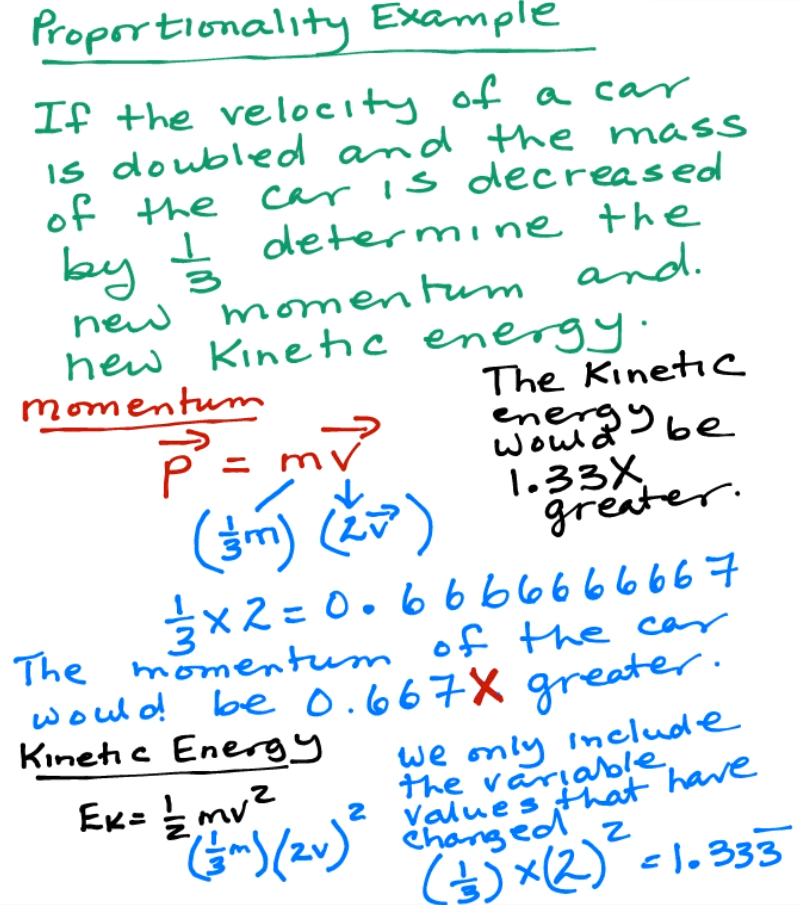
\includegraphics[width=0.45\textwidth]{q-prop}
    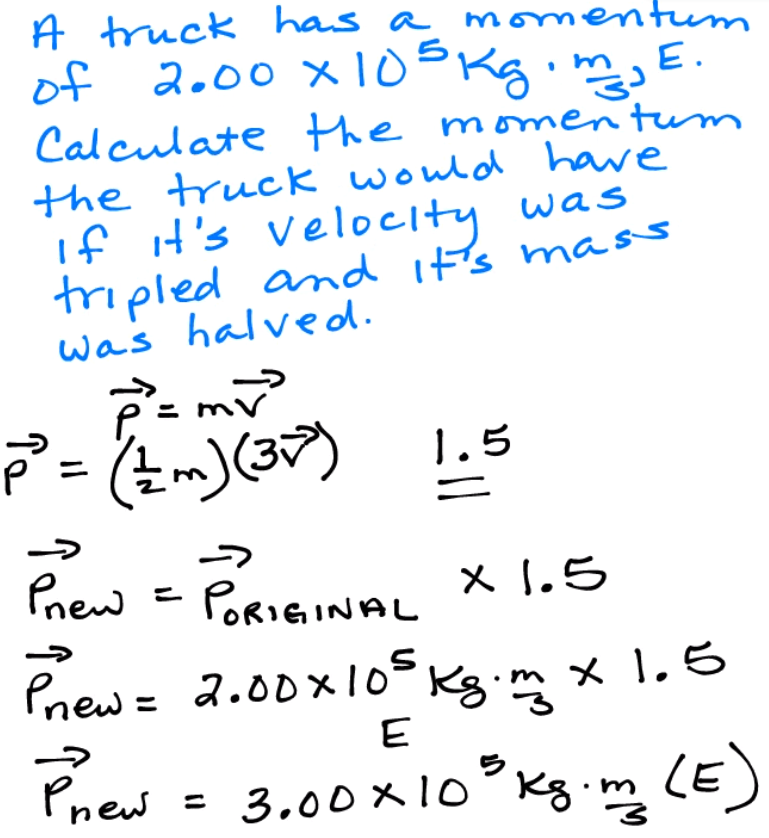
\includegraphics[width=0.45\textwidth]{q-prop-2}
\end{figure}

Tip: When determining how a variable changes proportional to the others in an equation, \hl{isolate the variable to one side}.

\subsection{Conventions}
\subsubsection{Signs}
\begin{itemize}
    \item{$+$ positive: right, up, north, east}
    \item{$-$ negative: left, down, south, west}
\end{itemize}

\subsubsection{Direction}
\begin{figure}[H]
    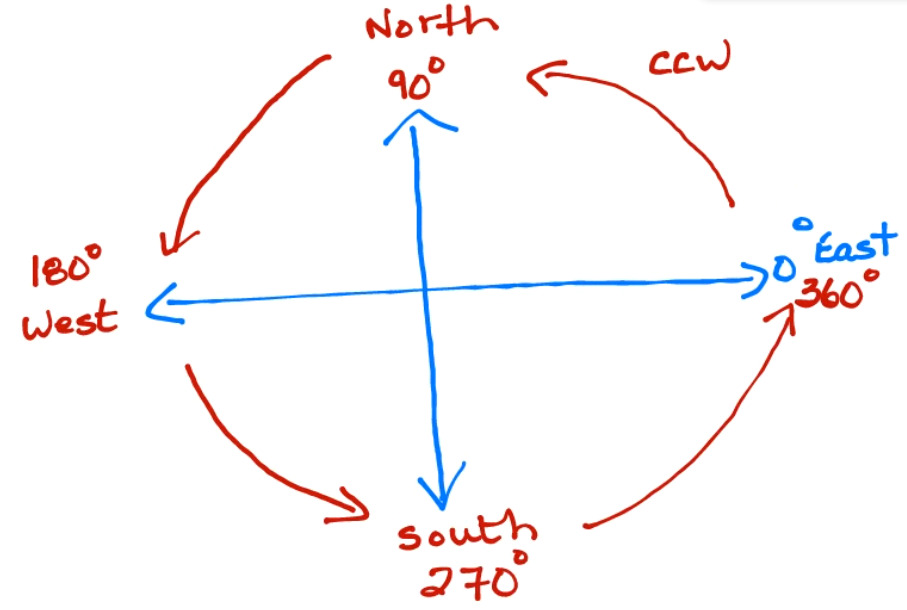
\includegraphics[width=0.75\textwidth]{direction}
\end{figure}

\subsubsection{Uniform Velocity}
$$v = \frac{d}{t}$$
Uniform = constant: velocity does not change over time.

If velocity changes (starts from rest, acceleration exists) then this formula CANNOT be used. There are others on your formula sheet.

\subsubsection{Formula Review}
$$g = \SI{9.81}{\m\per\s^2}$$

$$E_M = E_p + E_k$$
$$\sum{E_{top}} = \sum{E_{bottom}}$$
$$E_p + E_k = E_p + E_k$$

$$\textrm{Newton's 2nd Law (Force, in N)} = \vec{F} = m\vec{a}$$
$$\textrm{Weight (N)} = \vec{F_g} = m\vec{g}$$

\subsubsection{Inertia}
The tendency of an object to resist acceleration.

Object wants to maintain the velocity it was at --- e.g. stay at rest if suddenly moved, or keep moving forward if suddenly stopped.

e.g. Pulling the cover under a table fast enough doesn't drag everything with it. A large boulder being transported in a truck will smash into the driver if the truck suddenly stops.

\subsubsection{Angular Vector}
Angular vectors are composed of $x$ and $y$ components.
When given a vector with an angle, you will probably be given the value of the hypotenus.
Use trigonometry to solve for each component.

\pagebreak

\section{Momentum}
\Large $$\vec{p} = m\vec{v}$$ \normalsize

Momentum is conserved between colliding objects in a isolated/closed system.

\begin{itemize}
    \item{$\vec{p}$ = momentum, product of mass and velocity\\vector quantity, $\si{\kg\cdot\m\per\s}$ or $\si{\N\cdot\s}$}
    \item{$m$ = mass\\scalar quantity, $\si{\kg}$}
    \item{$\vec{v}$ = velocity\\vector quantity, $\si{\m\per\s}$}
\end{itemize}
\Large
$$\vec{p} \propto m$$
$$\vec{p} \propto \vec{v}$$
\normalsize

\subsection{Examples}
\begin{figure}[H]
    \centering
    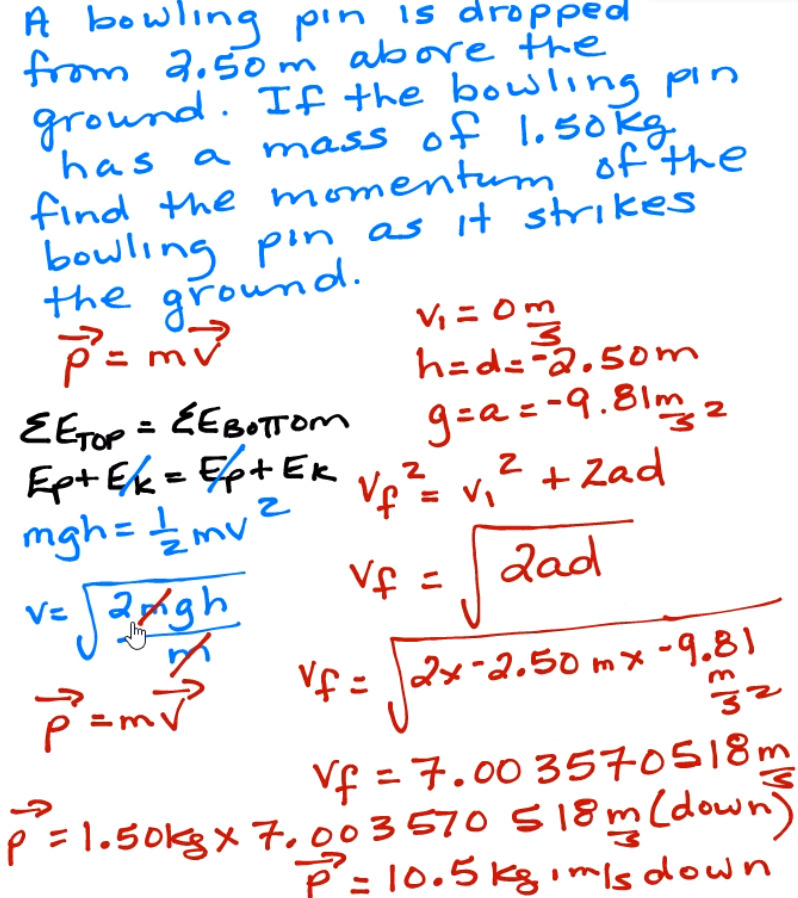
\includegraphics[width=0.75\textwidth]{q-mom}
\end{figure}
\begin{figure}[H]
    \centering
    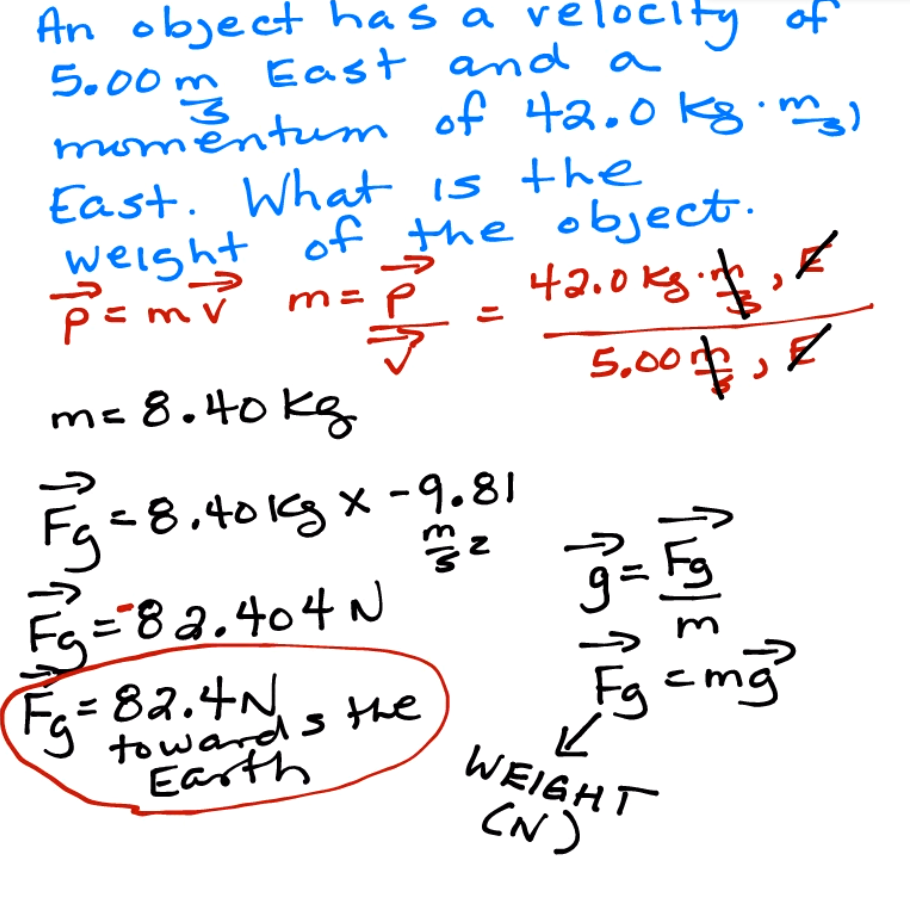
\includegraphics[width=0.75\textwidth]{q-mom-2}
\end{figure}
\begin{figure}[H]
    \centering
    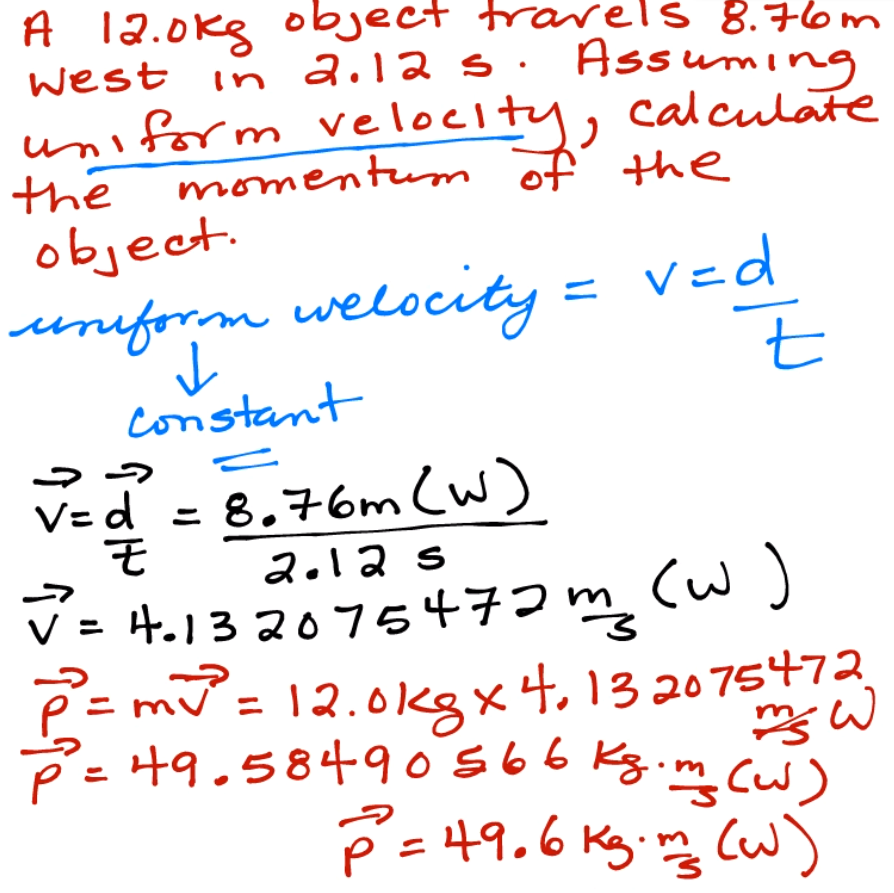
\includegraphics[width=0.75\textwidth]{q-mom-3}
\end{figure}

\section{Impulse}
\Large $$\Delta\vec{p} = \vec{p}_f - \vec{p}_i$$ \normalsize

Impulse is change in momentum; a \hl{force applied} to an object will \hl{change its momentum}.

\subsection{Formula}
\Large $$\Delta\vec{p} = \vec{F}\Delta{t} = m\Delta{\vec{v}}$$ \normalsize
$$\si{\kg\cdot\m\per\s} = \si{\newton\cdot\s} = \si{\kg\cdot\m\per\s}$$

Can be reorganized into Newton's 2nd law.
$$\vec{F} = \frac{m\Delta\vec{v}}{\Delta{t}} = m\Delta{a}$$
$$\vec{F} \propto \frac{1}{\Delta{t}}$$
Force is inversely proportional to time; a large force will be in small time (swift execution), a small force will be over large time.

\subsection{Application}
$$\vec{F} = \frac{\Delta\vec{p}}{\Delta{t}}$$

The greater the time is for an object to, say, fall and hit the ground, the impact will have less force, if all other variables are the same. By this logic, a more cushiony ground would cause the object to take more time to hit the ground, resulting in less force, cushioning their fall. The same applies to airbags.

\begin{figure}[H]
    \centering
    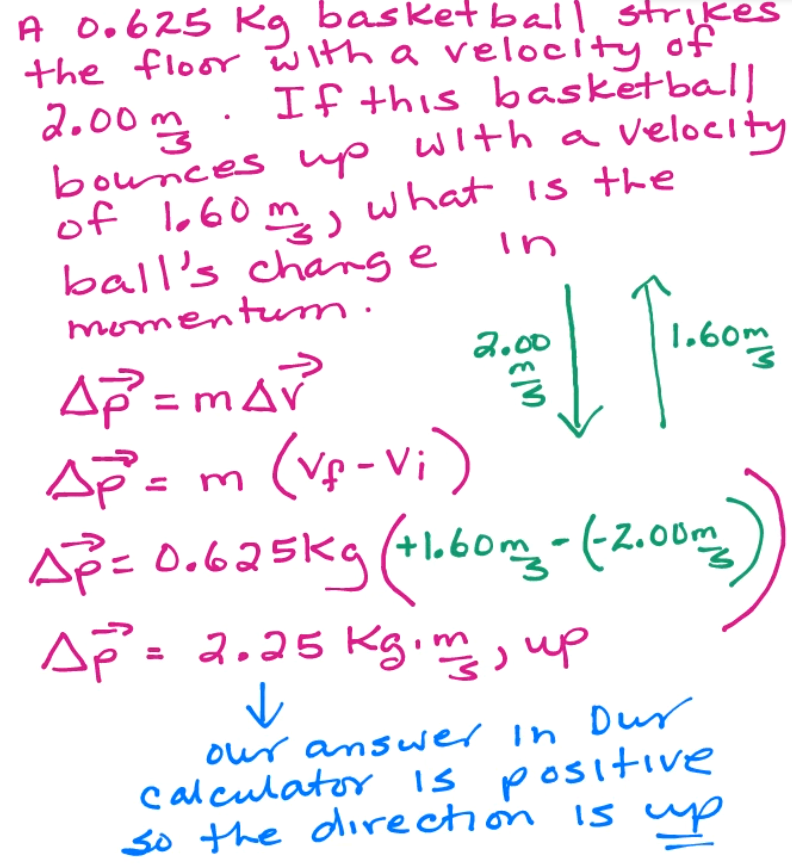
\includegraphics[width=0.4\textwidth]{q-imp}
\end{figure}
\begin{figure}[H]
    \centering
    \caption{A frictionless disc of mass \SI{0.500}{\kg} is moving in a straight line across an air table top at a speed of \SI{2.40}{\m\per\s} when the disc bumps into an elastic band stretched between two fixed posts. If the elastic band exerts an opposing force of \SI{1.40}{\N} on the disc for \SI{1.50}{\s}, calculate the final velocity of the disc.}
    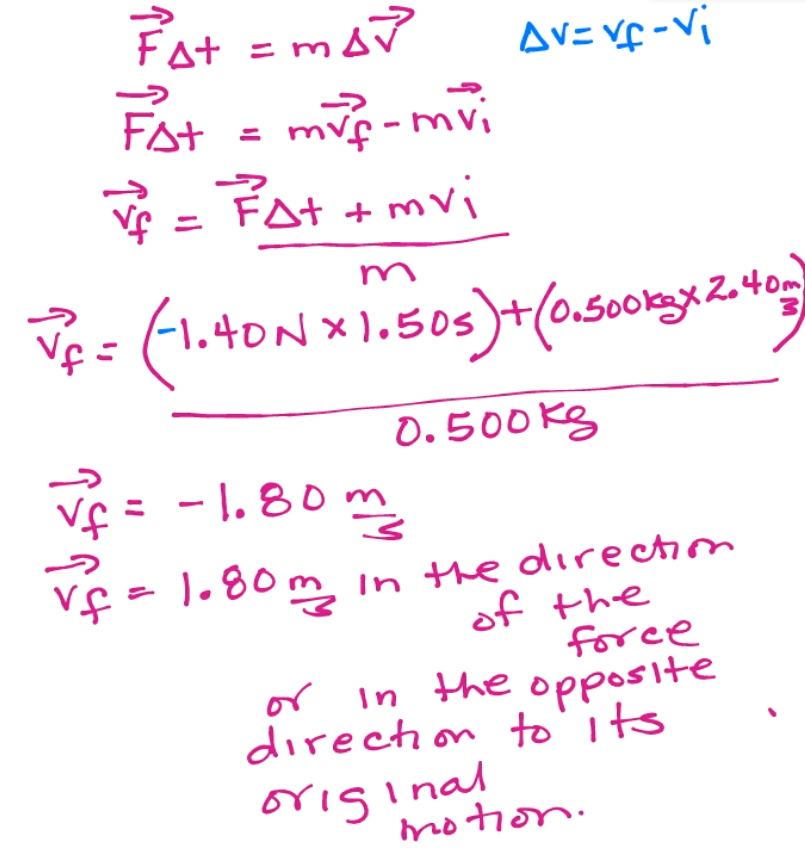
\includegraphics[width=0.8\textwidth]{q-imp-2}
\end{figure}

\pagebreak

\section{Force as a Function of Time Graphs}
\begin{itemize}
    \item{$y$-axis = Force ($\vec{F}$, $\si{\N}$)}
    \item{$x$-axis = Time ($t$, $\si{\s}$)}
    \item{Area under line = Change in momentum, aka. Impulse ($\Delta{\vec{p}}$, $\si{\N\cdot\s}$)}
\end{itemize}

\section{Conservation of Momentum (Collisions)}
\begin{itemize}
    \item{Momentum is used to analyze collisions and explosions}
    \item{Kinetic energy alone is not enough for analyzing an explosion/collision, because energy could be lost in the form of heat, light, or sound}
    \item{
        In an \hl{isolated system} ($F_{net} = 0$)
        \begin{itemize}
            \item{\hl{Momentum is conserved} during collisions and explosion ($\vec{p}_i = \vec{p}_f$)}
        \end{itemize}
    }
    \item{In a collision, impulse is provided to each object}
\end{itemize}

\subsection{Law of Conservation of Momentum}
\begin{itemize}
    \item{\textbf{Conservation}: to protect form loss or depletion}
    \item{The \hl{total linear momentum} of an isolated system remains \hl{constant} (it is conserved)}
    \item{An isolated system is one for which the \hl{vector sum} of the \hl{external forces} acting on the system is \hl{zero}}
\end{itemize}

\subsection{Elastic Collision}
$$\sum\vec{p} = \sum\vec{p}\,'$$
$$\vec{p}_1 + \vec{p}_2 = \vec{p}_1\,\!' + \vec{p}_2\,\!'$$
$$\textrm{momentum before collision} = \textrm{momentum after collision}$$

An elastic collision is a collision in which colliding objects rebound \hl{without lasting deformations} OR \hl{without the generation of heat}.

In an elastic collision, \hl{BOTH momentum and kinetic energy is conserved}.

To verify if a collision type is elastic, check to see if $E_k$ is conserved the same way as momentum above (before = after).
$$\sum E_{k_i} = \sum E_{k_f}$$
Don't forget that energy is scalar, so don't give the velocity a negative sign to try to give it direction.

There is no given formula for this, you must make one per question.

\subsection{Example}
\begin{figure}[H]
    \caption{A $\SI{1000}{\kg}$ car travelling at $\SI{20.0}{\m\per\s}$ EAST collides with a $\SI{3000}{\kg}$ truck that is stopped at a red light. Immediately following the collision, the $\SI{1000}{\kg}$ car is travelling at $\SI{10.0}{\m\per\s}$ WEST. Calculate the velocity of the truck and verify that this is an elastic collsion.}
    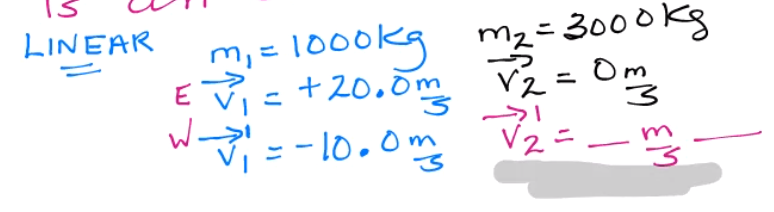
\includegraphics[width=0.6\textwidth]{q-elastic-1a}
    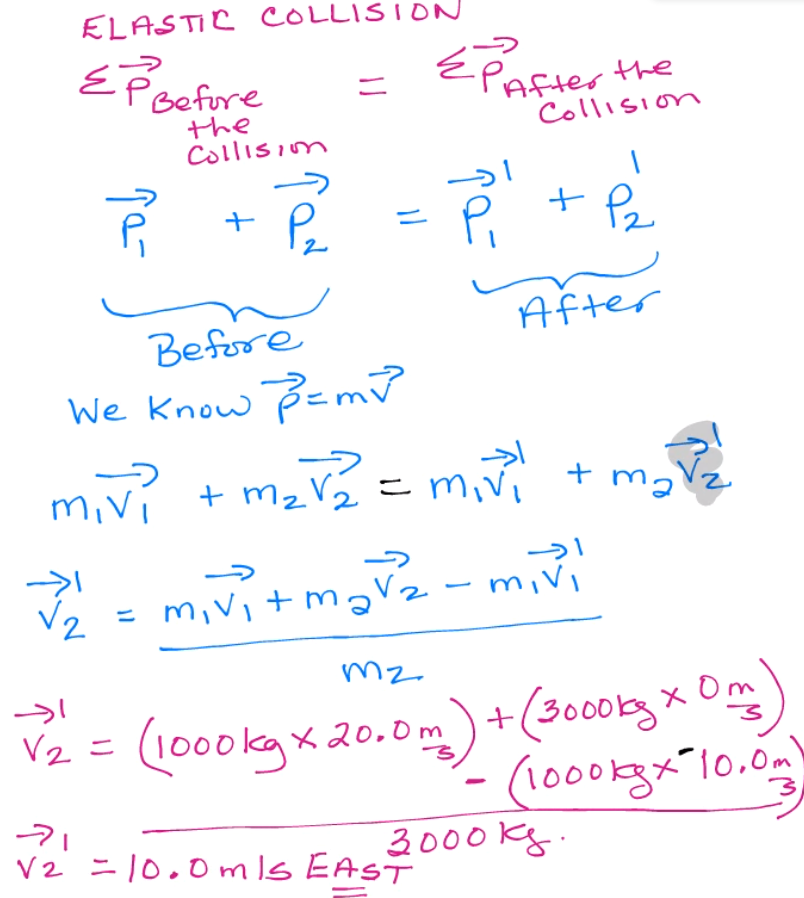
\includegraphics[width=0.6\textwidth]{q-elastic-1b}
    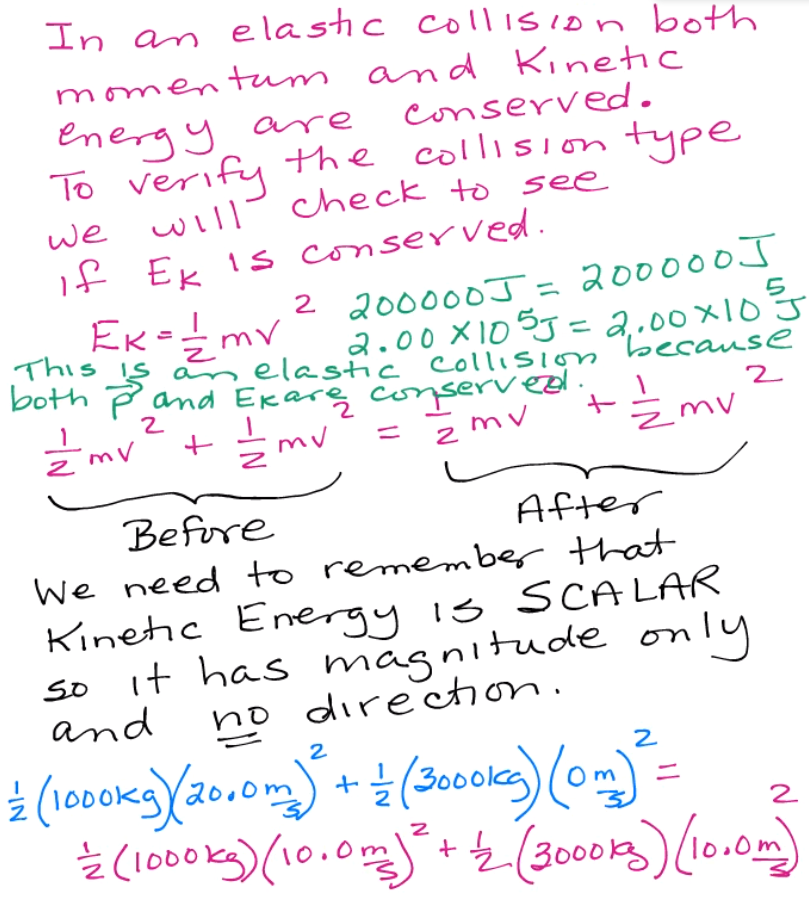
\includegraphics[width=0.5\textwidth]{q-elastic-1c}
    \centering
\end{figure}

\subsection{Example II (find mass)}
A proton with a mass of $\SI{1.67e-27}{\kg}$ moving $\SI{1.00e7}{\m\per\s}$ strikes a particle at rest and rebounds with a velocity of $\SI{6.00e6}{\m\per\s}$. If the unknown particle moves off with a speed of $\SI{4.00e6}{\m\per\s}$, what is the particle?
\begin{itemize}
    \item{electron = $\SI{9.11e-31}{\kg}$}
    \item{beta particle = $\SI{9.11e-31}{\kg}$}
    \item{alpha particle = $\SI{6.68e-27}{\kg}$}
\end{itemize}

\begin{figure}[H]
    \centering
    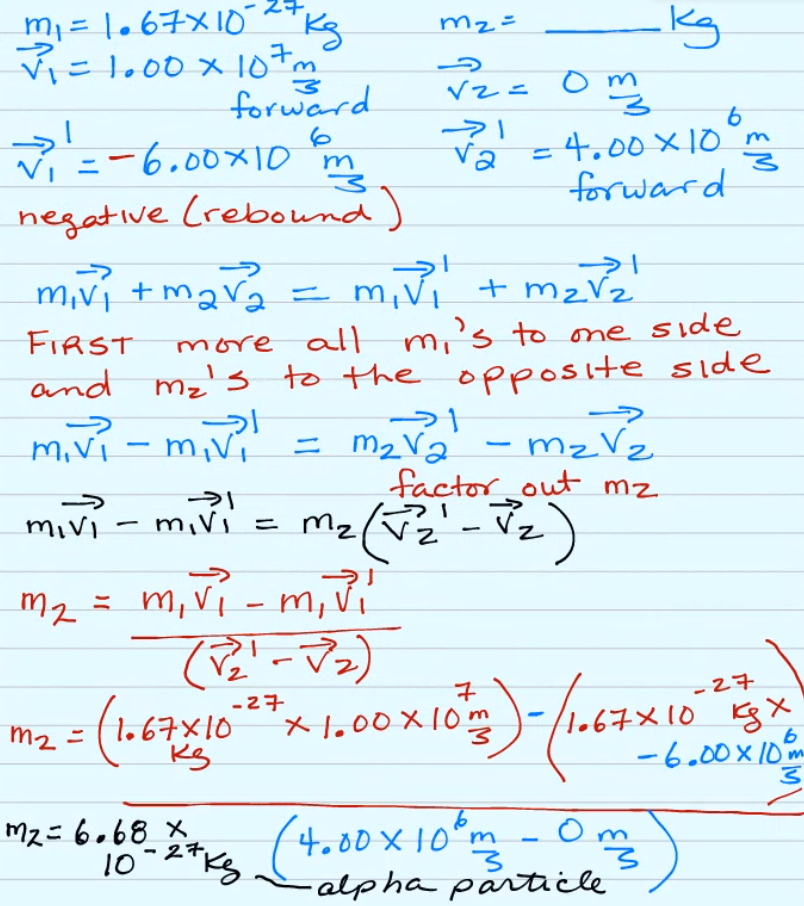
\includegraphics[width=\textwidth]{q-elastic-2}
\end{figure}

\subsection{Inelastic Collision}
\begin{itemize}
    \item{A collision in which the colliding objects become distorted/deformed and generate heat during the collision}
    \item{Objects crumple, dent, smash, couple --- join/stick together}
    \item{Momentum is conserved, \hl{kinetic energy is NOT conserved} ($\sum E_{k_i} \neq \sum E_{k_f}$)}
\end{itemize}
\Large $$m_1\vec{v_1} + m_2\vec{v_2} = (m_1+m_2)\vec{v}\,'$$ \normalsize
When objects couple, the mass of the objects will combine, and they will both share a velocity.

\subsubsection{Example}
\begin{figure}[H]
    \centering
    \caption{A $\SI{1000}{\kg}$ car travelling at $\SI{20.0}{\m\per\s}$ east collides with a $\SI{3000}{\kg}$ truck that is at rest. The two vehicles couple and move off together. Calculate the velocity of the car and truck after the collision.}
    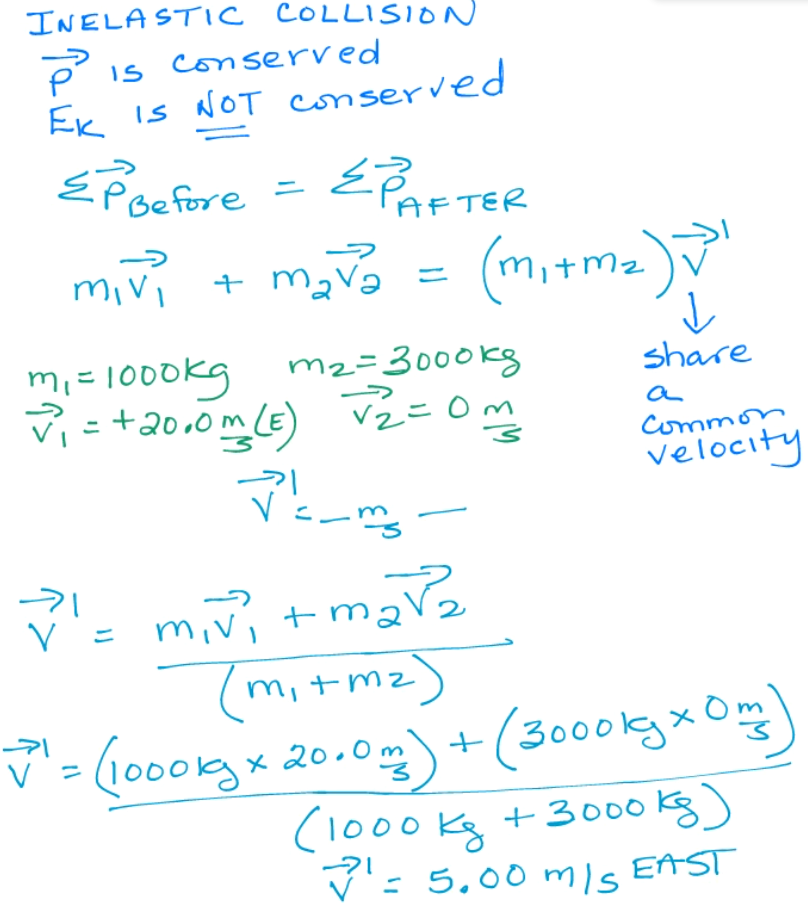
\includegraphics[width=0.5\textwidth]{q-inelastic-1}
    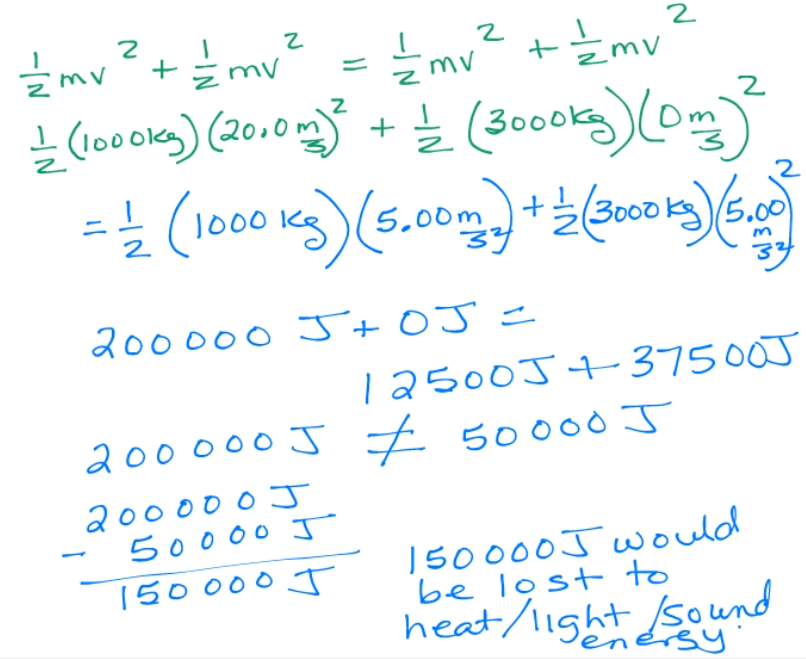
\includegraphics[width=0.5\textwidth]{q-inelastic-1b}
\end{figure}

\begin{figure}[H]
    \centering
    \caption{A $\SI{2452}{\kg}$ car travelling at $\SI{11.1}{\m\per\s}$ EAST collides with a $\SI{2682}{\kg}$ car travelling at $\SI{16.7}{\m\per\s}$ WEST. The two vehicles stick together. \\a) Calculate the resulting velocity of the two cars. \\b) Calculate the impulse experienced by the $\SI{2452}{\kg}$ car. \\c) Calculate the impulse experienced by the $\SI{2682}{\kg}$ car. \\d) Compare the impulses of the two vehichles.}
    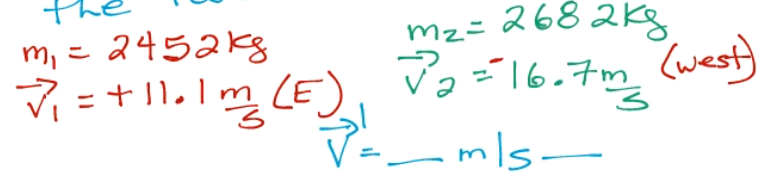
\includegraphics[width=0.5\textwidth]{q-inelastic-2}
\end{figure}
\begin{figure}[H]
    \centering
    \caption{a.}
    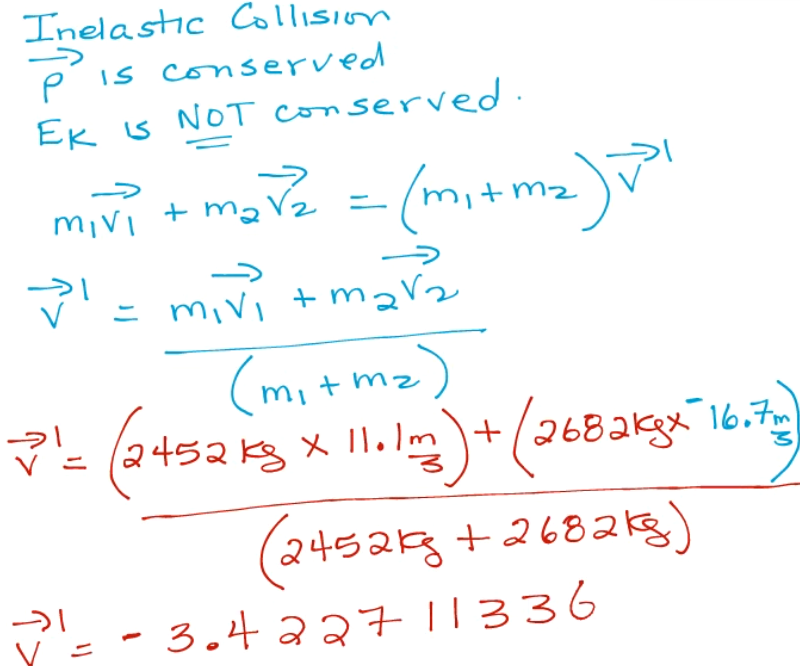
\includegraphics[width=0.50\textwidth]{q-inelastic-2b}
\end{figure}
\begin{figure}[H]
    \centering
    \caption{b. \& c.}
    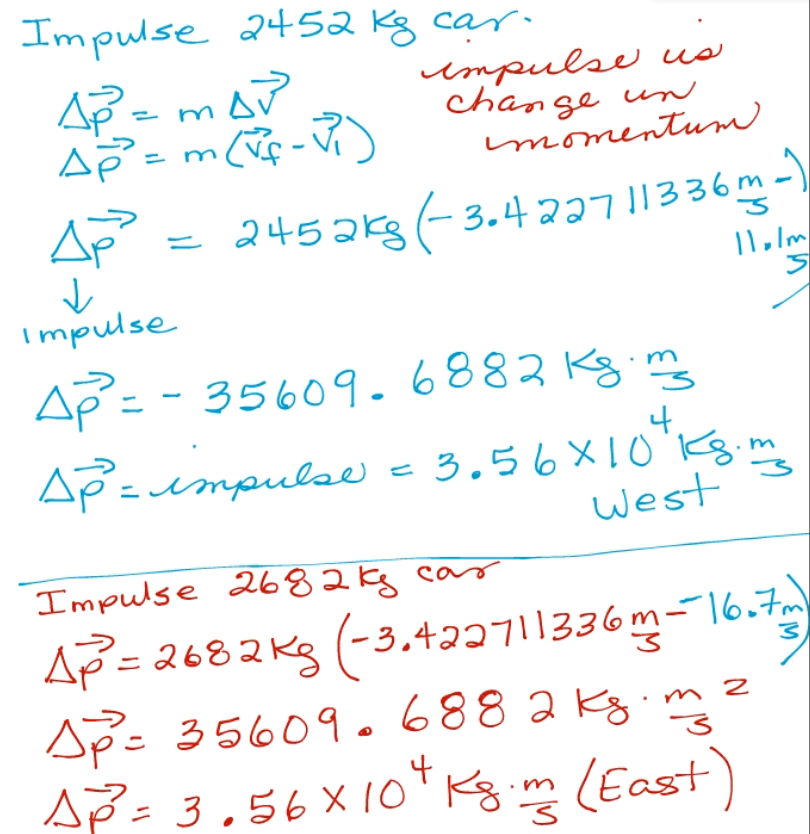
\includegraphics[width=0.50\textwidth]{q-inelastic-2c}
\end{figure}
d. The impulses are equal in magnitude, but in opposite directions.

\subsection{Collisions in Two Dimensions (Non-Linear)}
\begin{itemize}
    \item{The two forces colliding with one another combine to form the $x$ and $y$ component of after the collision, since momentum is conserved}
\end{itemize}
\subsubsection{Example}
\begin{figure}[H]
    \centering
    \caption{A $\SI{1000}{\kg}$ car travels EAST at $\SI{35.0}{\m\per\s}$. This car collides at an intersection with a $\SI{2000}{\kg}$ car travelling NORTH at $\SI{40.0}{\m\per\s}$. Calculate the velocity of the two stuck together vehicles after the collision.}
    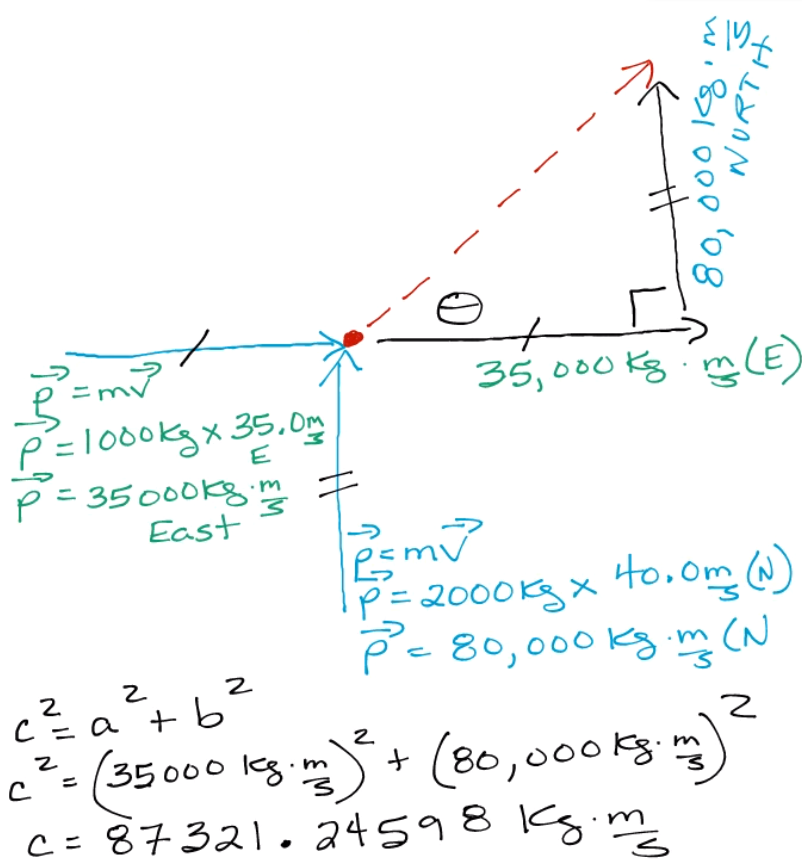
\includegraphics[width=0.45\textwidth]{q-2dcol}
    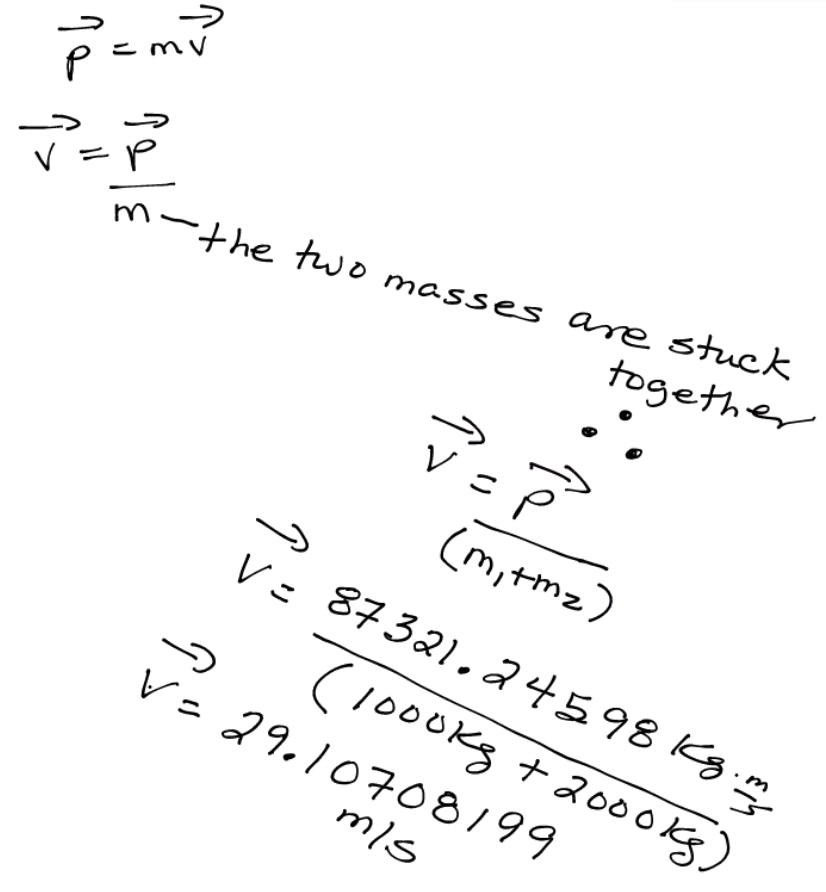
\includegraphics[width=0.45\textwidth]{q-2dcol-b}
\end{figure}
$$\tan{\theta} = \frac{ \SI{80000}{\kg\cdot\m\per\s}\textrm{(N)} }{ \SI{35000}{\kg\cdot\m\per\s}\textrm{(E)} }, \theta = \ang{66.37} \textrm{ N of E}$$

\pagebreak

\section{Recoil}
\begin{figure}[H]
    \centering
    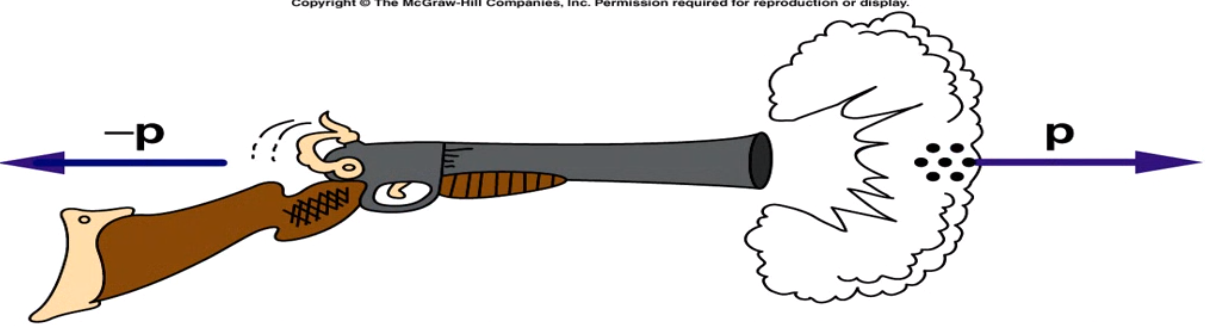
\includegraphics[width=\textwidth]{recoil}
\end{figure}
\begin{itemize}
    \item{aka. Kickback}
    \item{Backward momentum of a gun when it is discharged}
    \item{Recoil caused by the gun exactly balances the forward momentum of the projectile, accordings to Newton's 3rd Law}
    \item{\hl{The bullet and the gun experience an equal but opposite impulse}}
    \item{$\vec{p}$ is conserved}
    \item{$E_k$ is not conserved}
\end{itemize}

\subsection{Calculation}
\Large $$(m_1 + m_2)\vec{v}\,' = m_1\vec{v_1} + m_2\vec{v_2}$$ \normalsize
Objects start coupled/stuck together to begin with, but separate later.

Examples could be a person getting out of a canoe, or a person jumping off a skateboard, or two people pushing away from eachother.

\subsubsection{Example}
\begin{figure}[H]
    \centering
    \caption{If a $\SI{2.2}{\g}$ bullet is fired from a $\SI{3.00}{\kg}$ gun with a velocity of $\SI{452}{\m\per\s}$, what would be the resulting recoil velocity of the gun? ($\vec{v}_G = \SI{0.331}{\m\per\s}\textrm{ backward})$
}
    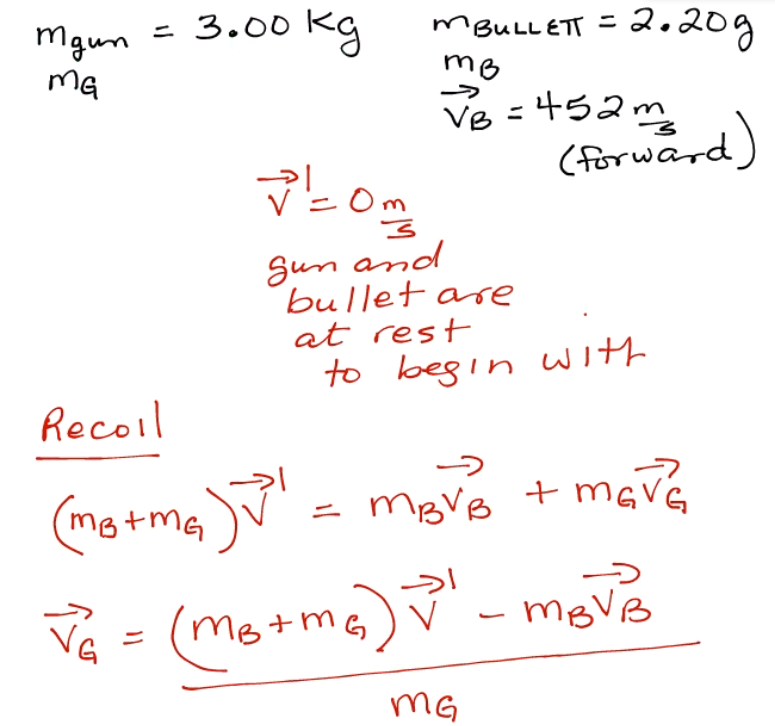
\includegraphics[width=0.4\textwidth]{q-recoil-1}
\end{figure}

\pagebreak

\section{Ballistic Pendulum}
\begin{figure}[H]
    \centering
    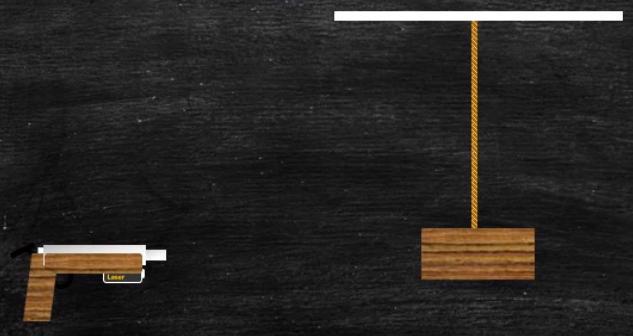
\includegraphics[width=0.50\textwidth]{ballistic}
\end{figure}
\begin{itemize}
    \item{Inelastic Collision}
    \item{Shooting a block of wood of known mass attached to a pendulum can be used to find the speed of a bullet}
    \item{Energy is conserved ($\sum{E_{bottom}} = \sum{E_{top}}$)}
\end{itemize}

\subsection{Example}
If the bullet has a mass of $\SI{7.50}{\g}$ and the pendulum has a mass of $\SI{2.50}{\kg}$ and rises to a height of $\SI{65.0}{\cm}$, find the speed of the bullet.

\begin{figure}[H]
    \centering
    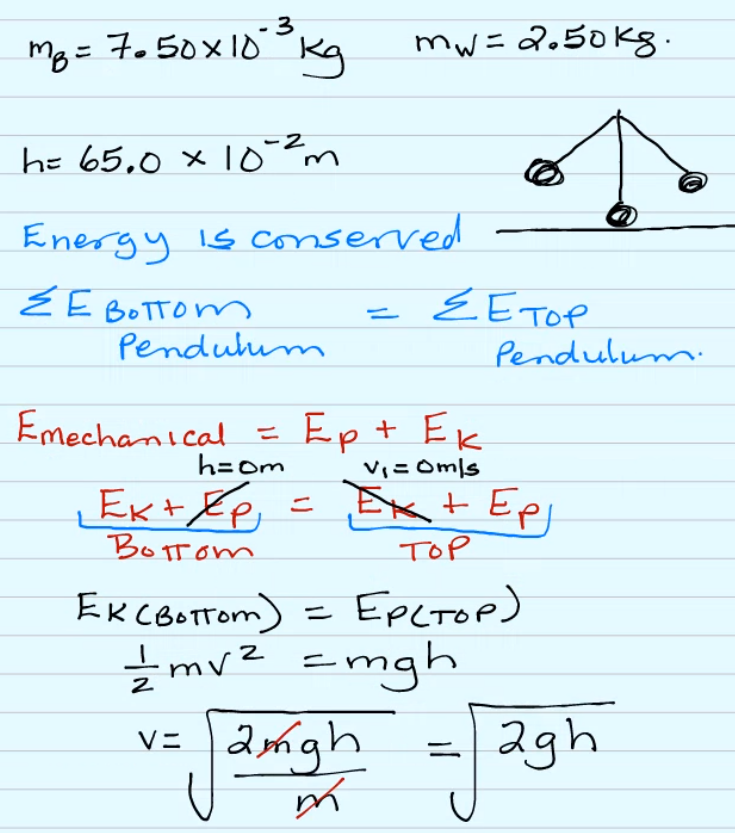
\includegraphics[width=0.6\textwidth]{q-pend-1a}
    \caption{This gives you velocity of bullet and pendulum stuck together. \\Solve for velocity of bullet using inelastic equation like before.}
\end{figure}

\section{Explosion}
\begin{itemize}
    \item{The \hl{initial momentum is (often) zero}, so the sum of the final momentums must be zero}
    \item{Energy is never conserved}
\end{itemize}

\subsection{Example}
A stationary bomb explodes into two fragments. The $\SI{1.70}{\kg}$ fragment flies off at $\SI{320}{\m\per\s}$, the other at $\SI{180}{\m\per\s}$. What is the mass of the bomb?

\begin{itemize}
    \item{$m_1 = \SI{1.70}{\kg}$}
    \item{$m_2 = \,?$}
    \item{$v_1 = \SI{320}{\m\per\s}$}
    \item{$v_2 = \SI{-180}{\m\per\s}$}
    \item{$\vec{v}\,' = 0$ (stationary)}
\end{itemize}

$$(m_1 + m_2)\vec{v}\,' = m_1\vec{v_1} + m_2\vec{v_2}$$
$$\frac{0 - m_1\vec{v_1}}{\vec{v_2}} = m_2$$
$$\frac{-(\SI{1.70}{\kg} \times \SI{320}{\m\per\s})}{\SI{-180}{\m\per\s}} = m_2$$

$$m_B = m_1 + m_2$$
$$m_B = \SI{1.70}{\kg} + \SI{3.02}{\kg} = \SI{4.72}{\kg}$$

\pagebreak

\subsection{Example II}
A $\SI{3.00}{\kg}$ bomb is flying through the air at $\SI{120}{\m\per\s}$ east when it explodes into two parts. The $\SI{1.40}{\kg}$ fragment flies off at $\SI{230}{\m\per\s}$ west. What is the velocity of the other fragment?

\begin{figure}[H]
    \centering
    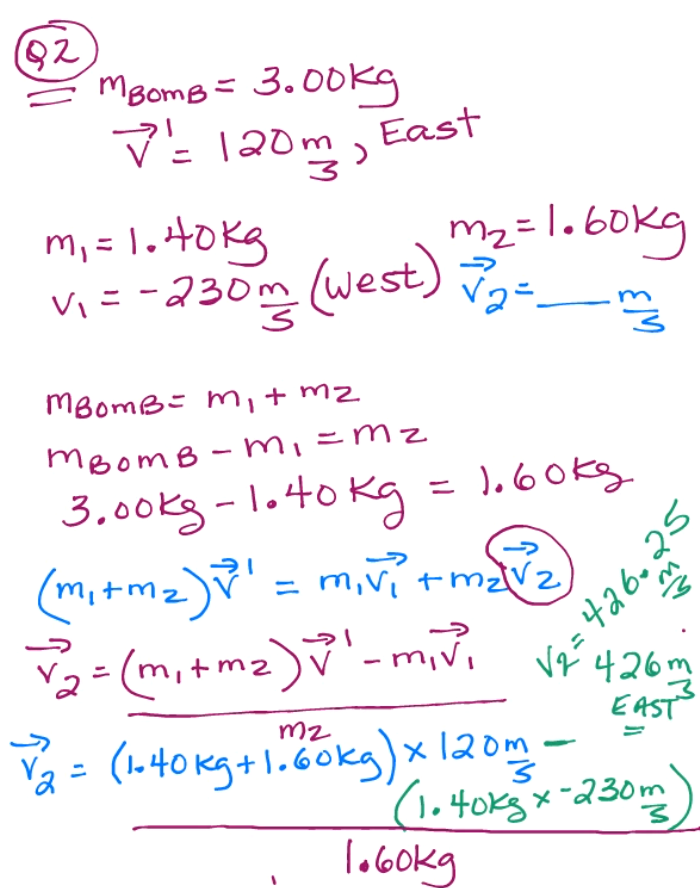
\includegraphics[width=0.8\textwidth]{q-explode-2}
\end{figure}

\pagebreak

\subsection{Example III}
A watermelon with a mass of $\SI{5.0}{\kg}$ spontaneously explodes. A mass of $\SI{1.5}{\kg}$ travels east at $\SI{6.0}{\m\per\s}$. What is the final velocity of the remaining $\SI{3.5}{\kg}$? 

\begin{itemize}
    \item{$m_1 = \SI{1.5}{\kg}$}
    \item{$m_2 = \SI{3.5}{\kg}$}
    \item{$\vec{v}\,' = 0$ (stationary)}
    \item{$\vec{v}_1 = \SI{6.0}{\m\per\s}$}
    \item{$\vec{v}_2 = \,?$}
\end{itemize}

\begin{figure}[H]
    \centering
    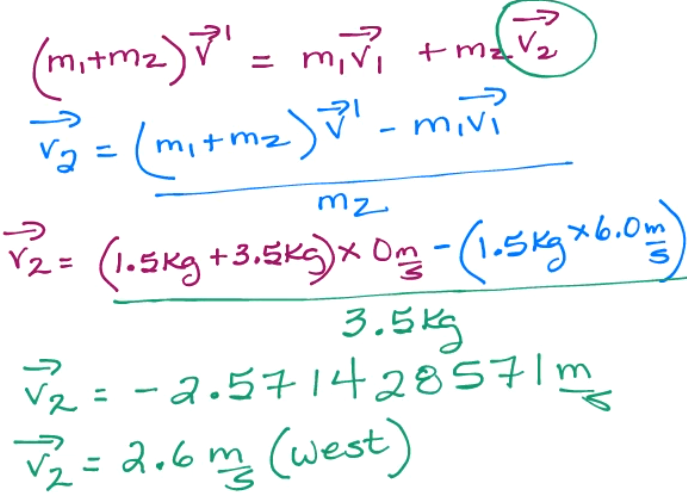
\includegraphics[width=0.75\textwidth]{q-explode-3a}
\end{figure}

Show that energy is not conserved in this explosion.
$$\sum{E_{k_i}} \neq \sum{E_{k_f}}$$
$$\frac{1}{2}mv^2 + \frac{1}{2}mv^2 \neq \frac{1}{2}mv^2 + \frac{1}{2}mv^2$$
$$\SI{0}{\J} + \SI{0}{\J} \neq \frac{1}{2}(\SI{1.5}{\kg})(\SI{6.0}{\m\per\s})^2 + \frac{1}{2}(\SI{3.5}{\kg})(\SI{2.571428571}{\m\per\s})^2$$
$$\SI{0}{\J} \neq \SI{39}{\J}$$
The kinetic energy after the explosion is greater than before, therefore kinetic energy was not conserved.

\pagebreak
\subsection{Example IV}
\begin{figure}[H]
    \centering
    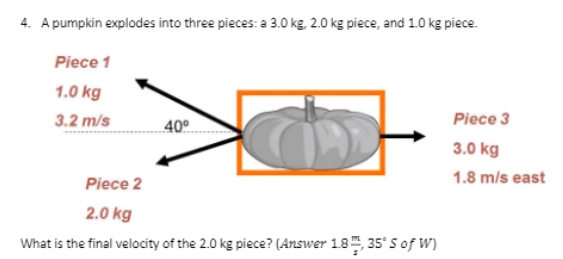
\includegraphics[width=0.50\textwidth]{q-explode-4}
\end{figure}
\begin{figure}[H]
    \centering
    \caption{Since Piece 1 is at an angle, you must calculate the components}
    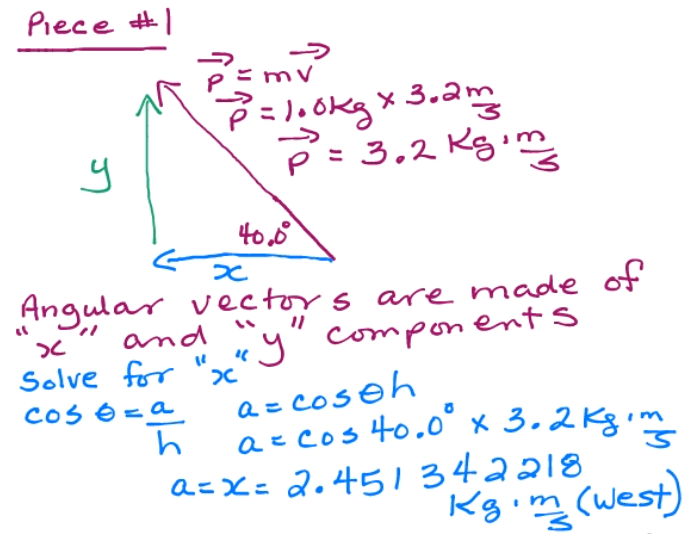
\includegraphics[width=0.50\textwidth]{q-explode-4a}
    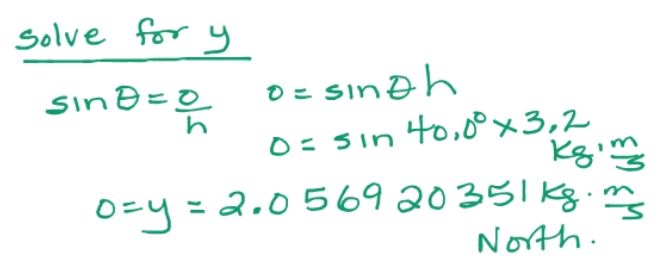
\includegraphics[width=0.50\textwidth]{q-explode-4b}
\end{figure}
\begin{figure}[H]
    \centering
    \caption{Piece 3 is not at an angle, so it's $y$ component is zero}
    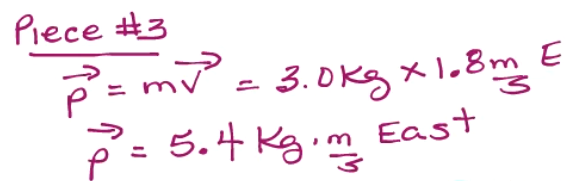
\includegraphics[width=0.50\textwidth]{q-explode-4c}
\end{figure}

\pagebreak
\begin{figure}[H]
    \centering
    \caption{Using conservation of momentum on each component to find Piece 2's $x$ and $y$ components}
    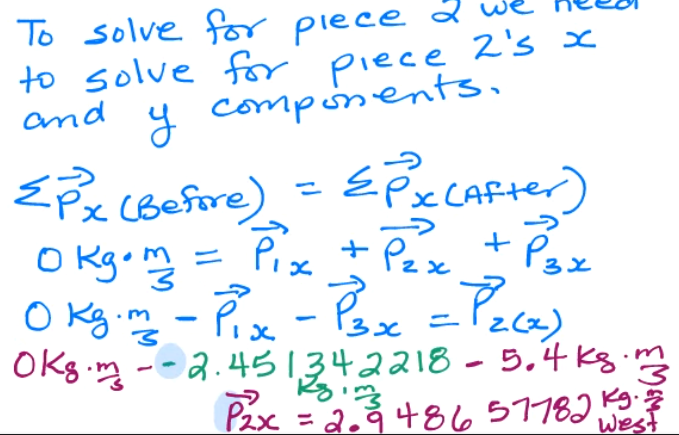
\includegraphics[width=0.50\textwidth]{q-explode-4d}
    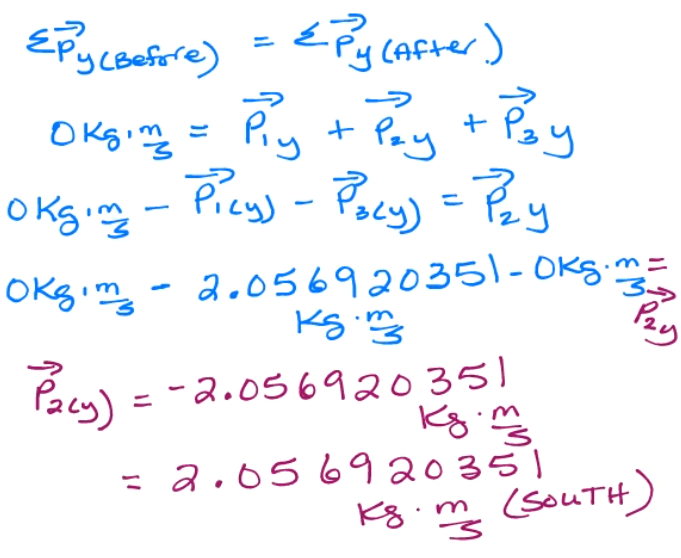
\includegraphics[width=0.50\textwidth]{q-explode-4e}
\end{figure}

\begin{figure}[H]
    \centering
    \caption{Pythagorem and Trig to calculate the answer magnitude and direction}
    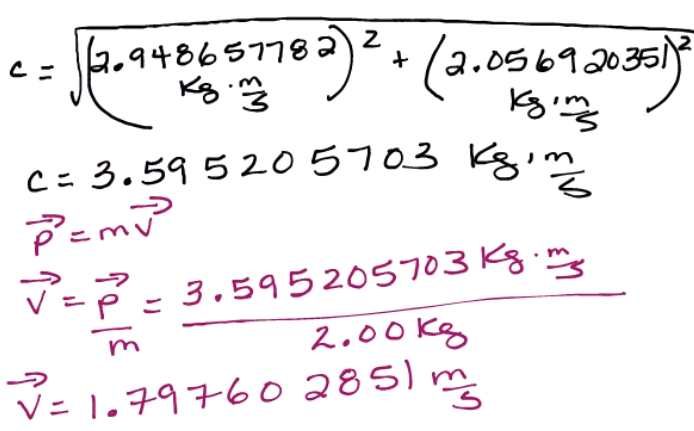
\includegraphics[width=0.50\textwidth]{q-explode-4f}
    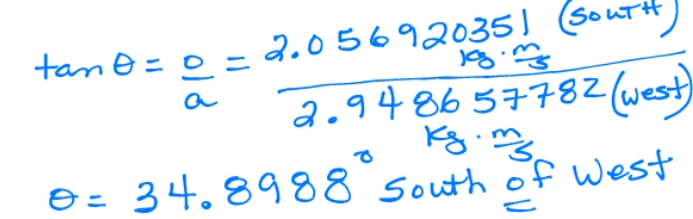
\includegraphics[width=0.50\textwidth]{q-explode-4g}
\end{figure}

\pagebreak
\section{Glancing Collision}
When objects don't hit straight on, rather bouncing off in different directions.

\subsection{Example}
A $\SI{10.0}{\kg}$ mass is moving East at an unknown velocity when it collides with a $\SI{7.50}{\kg}$ mass that is at rest. After the collision, the $\SI{10.0}{\kg}$ mass is traveling at a velocity of $\SI{4.00}{\m\per\s}, \ang{35.0}$ North of East, and the $\SI{7.50}{\kg}$ mass is traveling at a velocity of $\SI{6.12}{\m\per\s}, \ang{30.0}$ South of East. Calculate the velocity of the $\SI{10.0}{\kg}$ mass prior to the collision.

\begin{figure}[H]
    \centering
    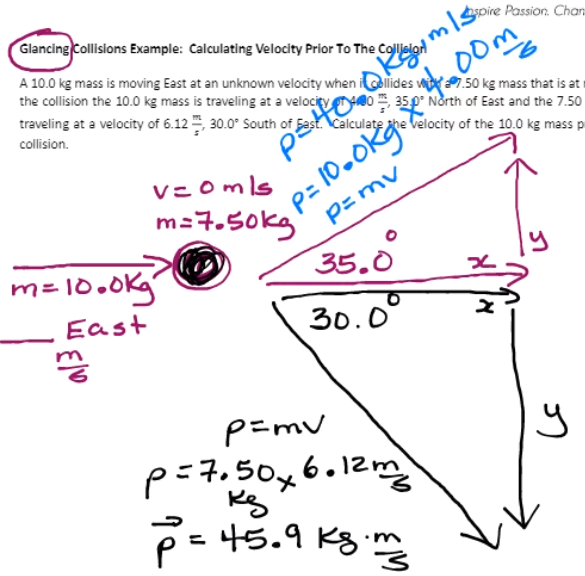
\includegraphics[width=0.8\textwidth]{q-glance-1a}
\end{figure}
\begin{figure}[H]
    \centering
    \caption{$x$ and $y$ components of $\SI{10.0}{\kg}$ mass}
    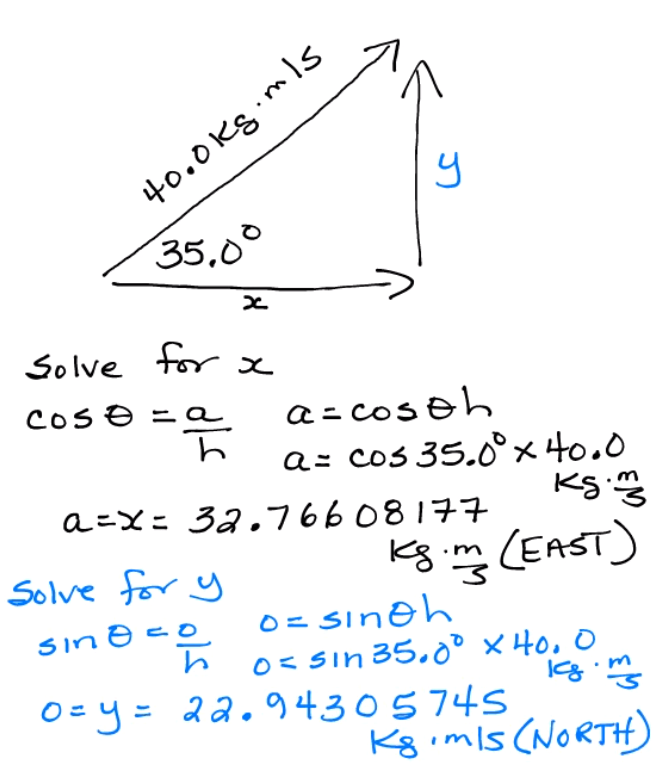
\includegraphics[width=0.55\textwidth]{q-glance-1b}
\end{figure}
\begin{figure}[H]
    \centering
    \caption{$x$ and $y$ components of $\SI{7.50}{\kg}$ mass}
    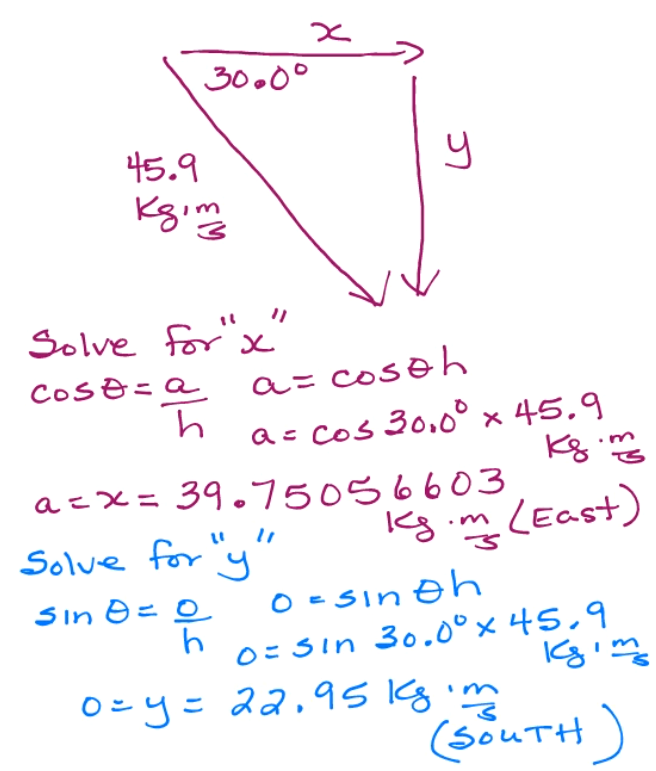
\includegraphics[width=0.55\textwidth]{q-glance-1c}
\end{figure}
\begin{figure}[H]
    \centering
    \caption{Side note: The $y$ components in this case must cancel out, since momentum is conserved, and there was zero $y$ momentum before the collision. (it's basically zero)}
    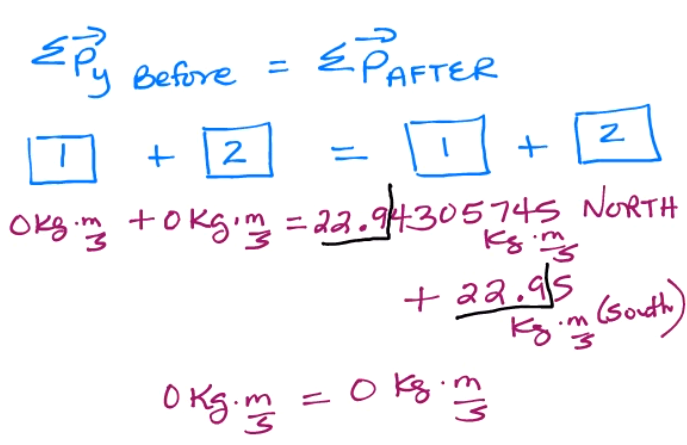
\includegraphics[width=0.50\textwidth]{q-glance-1d}
\end{figure}
\begin{figure}[H]
    \centering
    \caption{Using preservation of momentum to calculate the first object's momentum before the collision with the 2nd object}
    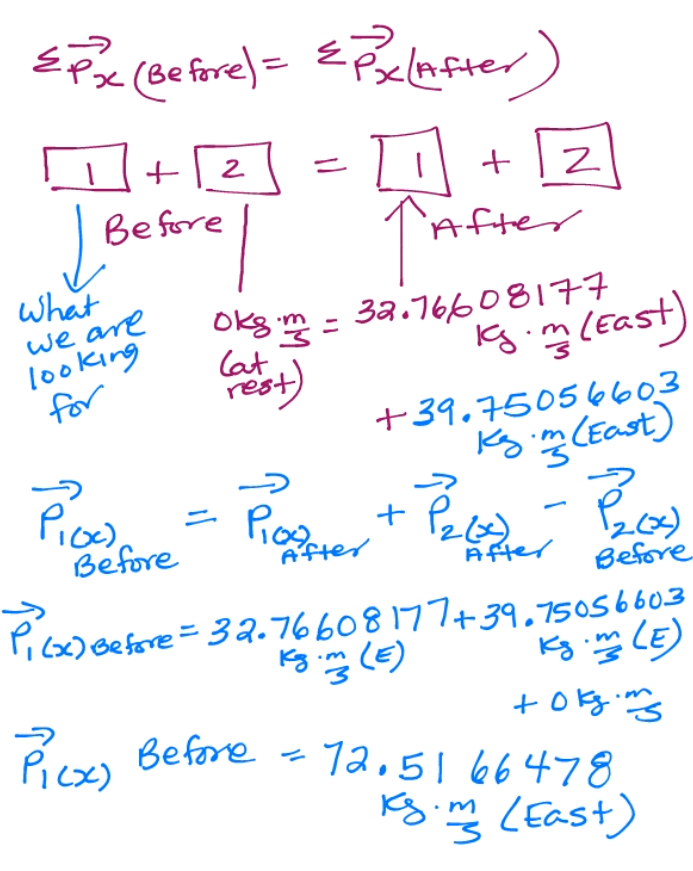
\includegraphics[width=0.50\textwidth]{q-glance-1e}
\end{figure}
$$\vec{v} = \frac{\vec{p}}{m}$$
$$\vec{v} = \frac{\SI{72.5}{\kg\cdot\m\per\s}}{\SI{10.0}{\kg}}$$
$$\vec{v} = \SI{7.25}{\m\per\s}\textrm{, EAST}$$

\end{document}
